\chapter{Integrals and Derivatives}
    \section{Fundamental Methods For Evaluating Integrals}
        To evaluate integrals numerically, we will use numerical approximations: the right Riemann sum, the left Riemann sum, or the trapezoidal rule.
        \begin{center}
            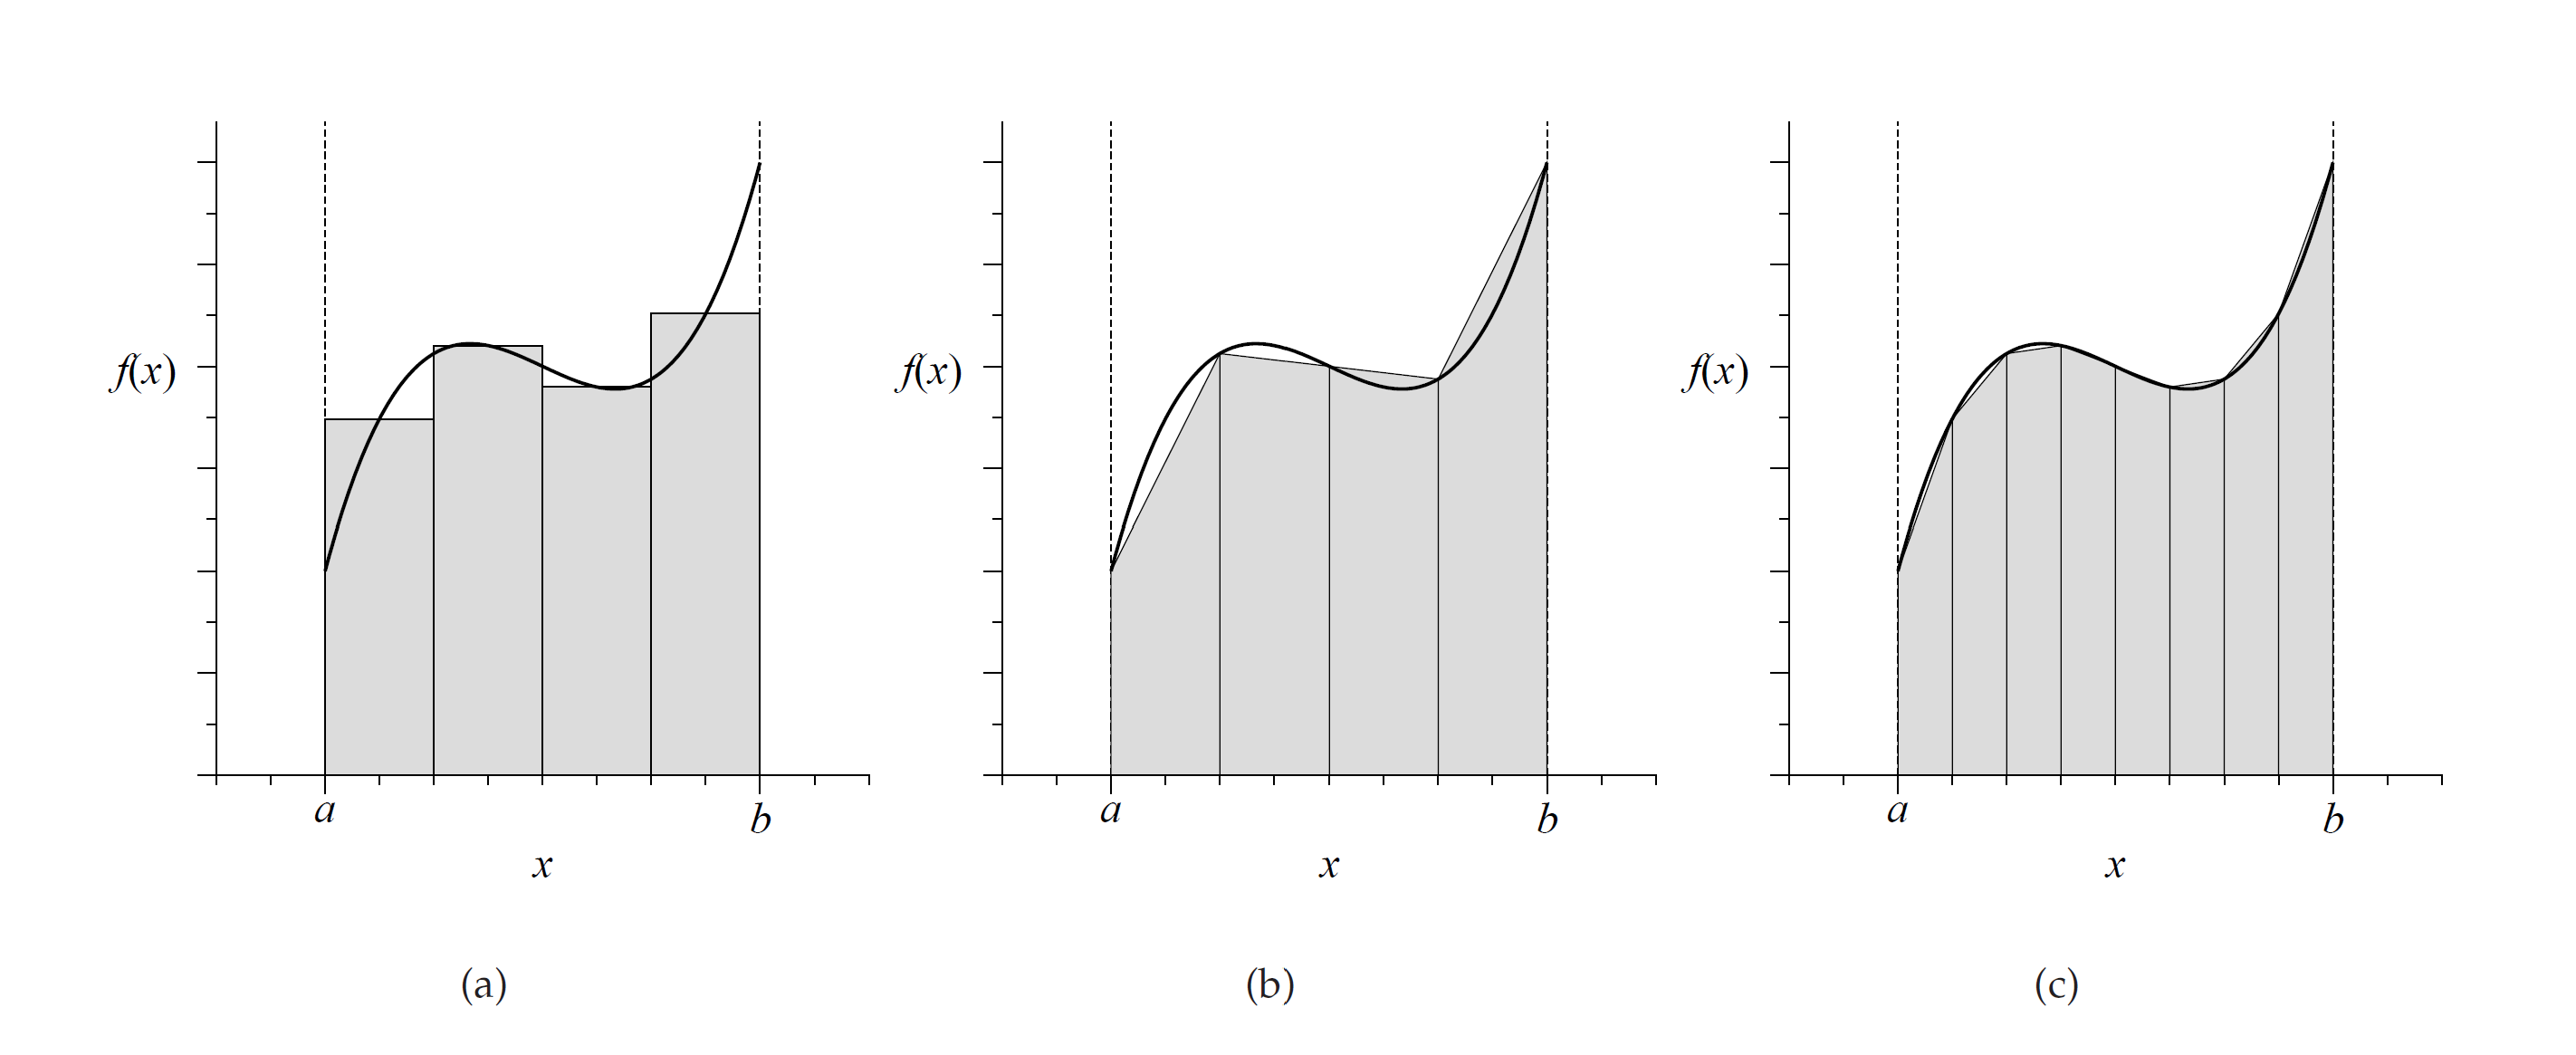
\includegraphics[width=300pt]{integral_approx.png}
        \end{center}
        \subsection{The Trapezoidal Rule}
            Suppose we have a function $f(x)$, let
            \begin{equation*}
                I(a, b) = \int_a^b f(x) dx
            \end{equation*}
            The trapezoidal rule is better than Riemann sums since it is closer to the correct area. Let's divide the interval from $a$ to $b$ into $N$ equal steps so each slice has a width $h = (b - a) / N$. The left and right sides of the trapezoid are $a + (k - 1) h$ and $a + kh$. So the area for slice $k$ is
            \begin{equation*}
                A_k = \frac{1}{2}h[f(a + (k - 1)h) + f(a + kh)]
            \end{equation*}
            Now, our approximation of $I(a, b)$ becomes
            \begin{align*}
                I(a, b) \simeq \sum_{k=1}^N A_k = \frac{1}{2}h \sum_{k=1}^N [f(a + (k - 1)h) + f(a + kh)] \\
                 = h[\frac{1}{2}f(a) + f(a + h) + f(a + 2h) + \dots + \frac{1}{2}f(b)] \\
                 = h[\frac{1}{2}f(a) + \frac{1}{2}f(b) + \sum_{k=1}^{N-1}f(a + kh)]
            \end{align*}
            This is an \textit{extended trapezoidal rule}.
        \subsection{Simpson's Rule}
            Simpson's rule has a greater accuracy than the trapezoidal rule, but it is slightly more complex. It can achieve the same and higher accuracy as the trapezoidal rule with fewer steps. 
            \newline \indent
            Simpson's Rule uses involves using three points to estimate a curve using a quadratic through those points and then you can find the area under those curves and sum them for an integral approximation. 
            \begin{center}
                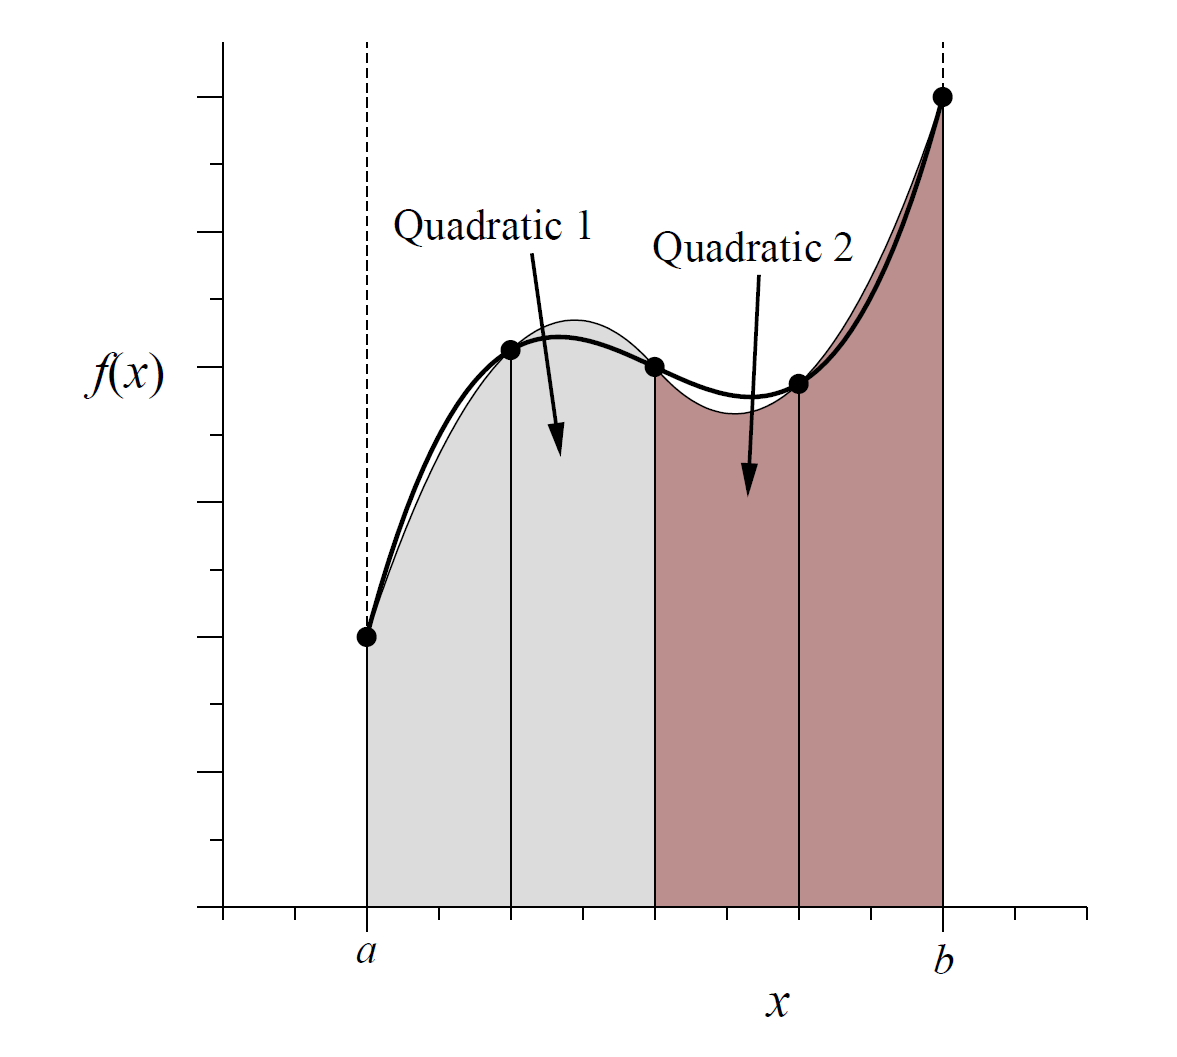
\includegraphics[width=200pt]{simpsons_rule.png}
            \end{center}
            If we call the spacing between adjacent points $h$. So for the purposes of the argument we will consider the points $x = -h$, $x = 0$, and $x = h$. If we fit a quadratic $Ax^2 + Bx + C$ to these points:
            \begin{equation*}
                f(-h) = Ah^2 - Bh + C, \qquad f(0) = C, \qquad f(h) = Ah^2 + Bh + C
            \end{equation*}
            Solving for $A$, $B$, and $C$, we get
            \begin{equation*}
                A = \frac{1}{h^2}[\frac{1}{2}f(h) - f(0) + \frac{1}{2}f(-h)] \qquad B = \frac{1}{2h}[f(h) - f(-h)] \qquad C = f(0)
            \end{equation*}
            The area under this curve from $-h$ to $h$ is the integral of this polynomial
            \begin{equation*}
                \int_{-h}^h (Ax^2 + Bx + C) dx = \frac{2}{3}Ah^3 + 2Ch = \frac{1}{3}h[f(-h) + 4f(0) + f(h)]
            \end{equation*}
            This is \textit{Simpson's Rule}, which give an approximation to the area under to adjacent slices of our function. This formula only depends on the points and $h$ so we do not need to worry about fitting the curve every time. We can use this even if the points do not surround 0 since sliding the area side to side does not matter.
            \newline \indent
            For a general integral we must combine successive pairs of two slices to form that entire area.
            \begin{align*}
                I(a, b) \simeq \frac{1}{3}h[f(a) + 4f(a + h) + f(a + 2h)] + \\
                    \frac{1}{3}h[f(a + 2h) + 4f(a + 3h) + f(a + 4h)] + \dots \\
                    \frac{1}{3}h[f(a + (N - 2)h) + 4f(a + (N - 1)h) + f(b)]
            \end{align*}
            which becomes
            \begin{equation*}
                I(a, b) \simeq \frac{1}{3}h[f(a) + f(b) + 4\sum_{k=1}^{N/2}f(a + (2k - 1)h) + 2\sum_{k=1}^{N/2 - 1}f(a + 2kh)]
            \end{equation*}
            This is called the \textit{extended Simpson's Rule}.